\chapter{Superficies. Primera forma fundamental y cálculo tensorial}

\section{Concepto de superficie}
\large 

Un subconjunto $S\subseteq \mathbb{R}^3$ es una \emph{superficie regular} de $\mathbb{R}^3$ si para cada punto $P\in S$ existe un conjunto abierto de $\mathbb{R}^2$, $U\subseteq \mathbb{R}^2$, un conjunto abierto $V\subseteq \mathbb{R}^3$ y una aplicación:
\begin{align*}
    \mathbf{x}:U\subseteq \mathbb{R}^2 &\longrightarrow V \cap S\\
    (u,v)& \longmapsto \mathbf{x}(u,v)=(x(u,v),y(u,v),z(u,v))
\end{align*}
tal que:
\begin{enumerate}
    \item[(i)] $\mathbf{x}:U\rightarrow V\cap S$ es de clase $C^\infty (U)$, (es decir, $x((u,v), y(u,v), z(u,v))$ son funciones de clase $C^\infty $ en su dominio).

    \item[(ii)] $\mathbf{x}:U\rightarrow V\cap S$ es un \emph{homomorfismo}, es decir, es \emph{biyectiva} (uno a uno), y su aplicación inversa es continua (esta condición evita que la superficie tenga auto intersecciones). 

    \item[(iii)] $\mathbf{x}:U\rightarrow V\cap S$ es \emph{regular}, es decir, su imagen es bidimensional, si la matriz jacobiana de derivadas es de rango 2 en $U$.
    $$
    J(u,v)=D\mathbf{x}=\left ( 
    \begin{array}{cc}
         \pdv{x(u,v)}{u}&\pdv{x(u,v)}{v}  \\\\
         \pdv{y(u,v)}{u}&\pdv{y(u,v)}{v}  \\\\
         \pdv{z(u,v)}{u}&\pdv{z(u,v)}{v}
    \end{array}
    \right )\longrightarrow rg(J)=2 \ , \ \forall (u,v)\in \mathbb{R}^2
    $$

    Esta condición evita que tengamos casos degenerados, como puntos o rectas (por ejemplo: $\mathbf{x}(u,v)=(u+v,u+v,u+v)$, que es en realidad una recta $\mathbf{x}(t)=(t,t,t)$).
\end{enumerate}

\paragraph{Notación:} Al par $(U,\mathbf{x}(u,v))$ se le denomina \emph{carta} (o entorno) local de la superficie $S$ (típicamente en torno a un punto $P \in S$). La carta proporciona un sistema de coordenadas a través de una parametrización local de la superficie.
\newpage
\begin{wrapfigure}{l}{0.43\textwidth}
    \centering
    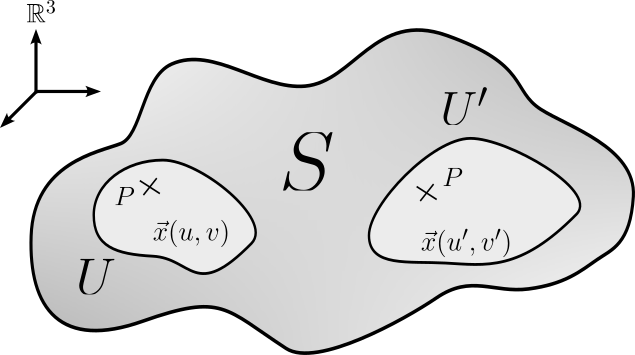
\includegraphics[scale=.4]{FOTOS/carta.png}
\end{wrapfigure}

La suma de todas las cartas que permiten cubrir completamente una superficie se conoce como \emph{atlas}. \\

Una superficie como $\mathbb{R}^2$ puede cubrirse mediante un atlas con una única carta (se conoce como superficie trivial). Si esta no es trivial, puede que hagan falta más de una carta para cubrir la superficie entera, como en el caso de la esfera o del cono, como se verá en el siguiente ejemplo.\\

\begin{mybox}
    \underline{Ejemplo A:} \\
        (i) El plano $XY$ puede cubrirse con una única carta:
        
        \begin{wrapfigure}{r}{0.25\textwidth}
            \centering
            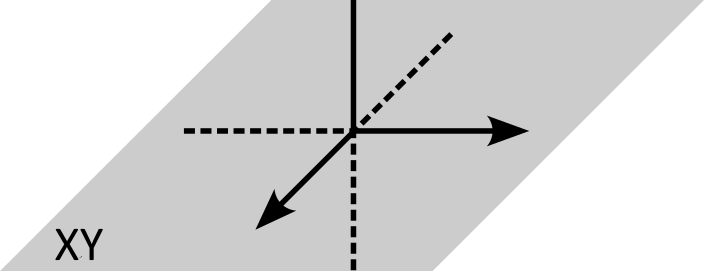
\includegraphics[scale=.2]{FOTOS/ejemplo2_A.png}
            \caption*{(i)}
        \end{wrapfigure}
        
        \begin{gather*}
        \mathbf{x}(u,v)=(u,v,0) \ , \text{con }u,v \in \mathbb{R}\\
        J(u,v)=\left ( \begin{array}{cc}
             1&0  \\
             0&1  \\
             0&0
        \end{array} \right ) \longrightarrow rg(J)=2 \ ; \ \forall u,v 
        \end{gather*}
        Lo mismo ocurre con las gráficas de las funciones de dos variables (representación en la carta de Monge):
        \begin{align*}
            f:U\subseteq \mathbb{R}^2 &\longrightarrow\mathbb{R}^3\\
                                 (x,y)&\longmapsto f(x,y)  \implies \mathbf{x}(u,v)=(u,v,f(u,v)) \text{ que tiene } rg(J)=2
        \end{align*}
            \begin{wrapfigure}{l}{0.2\textwidth}
             \centering
             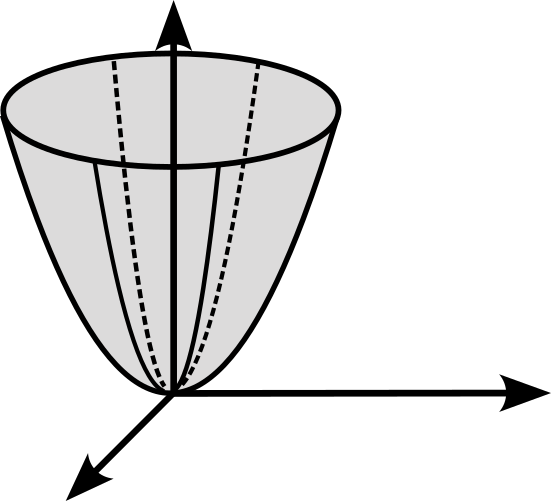
\includegraphics[scale=.18]{FOTOS/ejemplo2_A_2.png}
             \caption*{(ii)}
             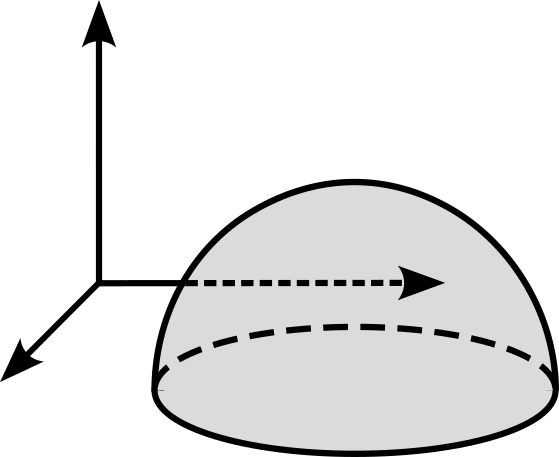
\includegraphics[scale=.18]{FOTOS/ejemplo2_A_4.png}
             \caption*{(iv)}
         \end{wrapfigure}
         (ii) El paraboloide de revolución $z=x^2+y^2$ se puede cubrir también con una carta:
        $$
        \mathbf{x}(u,v)=(u,v,u^2+v^2) \ , \ \text{con }u,v\in \mathbb{R} 
        $$
         (iii) El paraboloide hiperbólico $x=x^2-y^2$ se puede cubrir con la carta 
         $$\mathbf{x}(u,v)=(u,v,u^2-v^2)$$
         (iv) La semiesfera (\emph{hemisferio}) $z=\sqrt{1-x^2-y^2}$ (tomado de la esfera-- que \textbf{no} es una función--: $x^2+y^2+z^2=1$). Esta superficie \textbf{no} es regular a no ser que eliminemos de su dominio el ecuador (ya que para que sea regular, sus derivadas tienen que estar bien definidas, algo que no pasa cuando $z=0$). En este caso, la carta es: 
         $$
         \mathbf{x}(u,v)=\left (u,v,\sqrt{1-u^2-v^2}\right ) \ , \ U=\{ (u,v)\in \mathbb{R}^2 :u^2+v^2<1 \}
         $$
         
         (v) El cilindro $S=\{ (x,y,z)\in \mathbb{R}^3:x^2+y^2=1 \}$ (en coordenadas cilíndricas):
         $$
         \mathbf{x}(u,v)=(\cos u , \sin u , v) \ , \ u \in (0,2\pi),v\in \mathbb{R}
         $$
\end{mybox}
\begin{mybox}
         Para cubrir el cilindro, es decir, el atlas del cilindro, hacen falta \emph{dos} cartas (la razón es que el cilindro no se parece a $\mathbb{R}^2$ al tener una recta en la que está multievaluada. Esto implica que hagan falta operaciones para convertirlo en algo semejante a $\mathbb{R}^2$). \emph{No obstante, si se elimina una recta del cilíndro sí que puede cubrirse con una carta.}\\
         %AÑADIR DIBUJO

         (vi) La esfera $x^2+y^2+z^2=1$ implica que se necesitan seis cartas para cubrir el atlas, pero si usamos coordenadas esféricas necesitamos dos.
         $$
         \left \{ 
         \begin{array}{ccc}
             x &=& \pm \sqrt{1-y^2-z^2} \\
             y &=& \pm \sqrt{1-x^2-z^2} \\
             z &=& \pm \sqrt{1-x^2-y^2} \\
         \end{array}
         \right . \Longrightarrow\left \{
         \begin{array}{c}
              \mathbf{x}(u,v)=(\sin u \cos v, \sin u \sin v , \cos u)  \\
              U=\left \{ (u,v)\in \mathbb{R}^2:
              \begin{array}{c}
                   0<v<2\pi   \\
                   0<u<\pi 
              \end{array}
              \right \}
         \end{array} \right .
         $$

         %AÑADIRDIBUJOOOOO

         (vii) Cono: $S=\left \{ (x,y,z)\in \mathbb{R}^3: z=\sqrt{x^2+y^2} \right \}$. Esta superficie tiene un problema de derivabilidad en el origen de coordenadas (pico), por lo que \textbf{no} es regular en ese punto. Para construir una carta de la superficie podemos trabajar en coordenadas cilíndricas. En este caso necesita dos cartas \footnote[1]{Como con el cilindro, puede cubrirse con una carta si se elimina una recta.}:
         $$
         \mathbf{x}(u,v)=(u\cos v, u\sin v , v), \qquad 0<u<\infty , 0<v<2\pi 
         $$

         (viii) Helicoide (escalera de caracol): $\mathbf{x}(u,v)=(u \cos v, u\sin v, v$, con $0<u<\infty $ y $v\in \mathbb{R}$.

         %DIBUJOOOO
\end{mybox}


\section{Curvas en una superficie}
%DIBUJOOO

Sea una superficie regular $S$ y una carta local $(U,\mathbf{x}(u,v))$ de dicha superficie; y sea la aplicación $\mathbf{\sigma}$,
\begin{align*}
    \mathbf{\sigma}:I\in \mathbb{R}&\longrightarrow U\subseteq \mathbb{R}^2\\
    t&\longmapsto \mathbf{\sigma}(t)=(u(t),v(t)),
\end{align*}
suficientemente suave, es decir, de clase $C^r$ con $r\ge 1$ en el intervalo $I$. La aplicación $\mathbf{\sigma}(t)$ representa una curva dentro de la superficie S, en concreto dentro de $U$. 
$$
\mathbf{x}(u(t),v(t))=(x(u(t),v(t)),y(u(t),v(t)),z(u(t),v(t)))
$$
\subsection{Curvas coordenadas y coordenadas curvilíneas}
Dado un punto $P(u_0,v_0)$ hay dos curvas importantes que pasan por él, que son las curvas \emph{paralelas a los ejes} $u,v$, y se conocen como \emph{curvas coordenadas}.\\

%AÑADIR DIBUJOOO

Las curvas coordenadas generan una malla que recubre completamente la superficie. Por otro lado, estas coordenadas $u,v$ son lo que se conoce como \emph{coordenadas curvilíneas} sobre la superficie $S$, asociadas a una cierta carta local $(U,\mathbf{x}(u,v))$.

\subsection{Vectores tangentes a la superficie $S$ y espacio o plano tangente}
En cada punto de $S$ hay dos valores únicos de $u$ y $v$, en el cual podemos definir dos vectores tangentes a la superficie, mediante las derivadas parciales direccionales, a lo largo de la dirección $\mathbf{x}_u$ (y lo mismo para la dirección $v$).
$$
\mathbf{x}_u=\pdv{\mathbf{x}}{u}=\left ( \pdv{}{u}x(u,v),\pdv{}{u}y(u,v), \pdv{}{u}z(u,v)\right )
$$

El rango del jacobiano $J$ es $rg(J)=2$ al estar en el espacio bidimensional.
$$
rg(J)=rg\left [ \left ( 
\begin{array}{cc}
     \pdv{x}{u}&\pdv{x}{v}  \\\\
     \pdv{y}{u}&\pdv{y}{v}  \\\\
     \pdv{z}{u}&\pdv{z}{v}
\end{array}
\right )\right ] \longrightarrow \text{\parbox{9cm}{Los vectores $\mathbf{x}_u, \mathbf{x}_v$ son linealmente independientes. Esto significa que definen un plano tangente a la superficie $S$ en $P(u,v)$.}}
$$

Además, su producto vectorial genera un vector perpendicular al plano tangente de la superficie (o a la superficie mismamente) en $P(u,v)$.
$$
\mathbf{n}=\frac{\mathbf{x}_u \wedge \mathbf{x}_v}{||\mathbf{x}_u \wedge \mathbf{x}_v||}
$$

%AÑADIR DIBUJOOO 
    
El conjunto de vectores $\{ \mathbf{x}_u,\mathbf{x}_v,\mathbf{n} \}$ es una base de $\mathbb{R}^3$, en cualquier punto de la superficie $S$. La base en principio \emph{no es ortogonal} (en general $\mathbf{x}_u\cdot \mathbf{x}_v\neq 0$).\\

\begin{mybox}
Los vectores $\mathbf{x}_u,\mathbf{x}_v$ son vectores \textbf{tangentes} a la superficie y definen un \textbf{espacio bidimensional} que es el plano tangente a la superficie en un punto $P$.
\begin{gather*}
T_p(S)=lin\{ \mathbf{x}_u,\mathbf{x}_v \} \ ,\\
\text{si $\mathbf{w}\in T_p(S)$: }\mathbf{w}=a\mathbf{x}_u+b\mathbf{x}_v \ ,\\
\{ \mathbf{x}_u,\mathbf{x}_v,\mathbf{n} \} \text{ es base de }\mathbb{R}^3\ .
\end{gather*}
\end{mybox}

Si tenemos una curva contenida en $S$, $\mathbf{x}(u(t),v(t))$, y pasa por un punto $P\in S$, entonces su vector tangente o velocidad puede escribirse como combinación lineal de la base.
\begin{equation*}
\begin{split}
\mathbf{x'}(t)&=\pdv{\mathbf{x}}{u}(u(t),v(t))\cdot \dv{u(t)}{t}+\pdv{\mathbf{x}}{v}(u(t),v(t))\cdot \dv{v(t)}{t}\\
          &=u'(t)\mathbf{x}_u+v'(t)\mathbf{x}_v
\end{split}
\end{equation*}

Esto significa que el vector velocidad está contenido en $T_p(S)$.
\paragraph{Notación:} Para volver más compacta la notación, hacemos el cambio:
$$
\left \{ 
\begin{array}{c}
     u\equiv u^1  \\
     v\equiv u^2 
\end{array}
\right .
$$
y la superficie queda parametrizada entonces es $\mathbf{x}(u^1,u^2)$. Los vectores de la base $T_p(S)$ los redefinimos de la siguiente manera:
$$
\left .
\begin{array}{c}
     \mathbf{x}_u=\mathbf{x}_{u^1}=\pdv{\mathbf{x(u^1,u^2)}}{u^1}\equiv \mathbf{x}_1  \\\\
     \mathbf{x}_v=\mathbf{x}_{u^2}=\pdv{\mathbf{x(u^1,u^2)}}{u^2}\equiv \mathbf{x}_2
\end{array} 
\right \} \implies \text{\parbox{7cm}{$\mathbf{x}_\alpha (u^1,u^2)$ representará las derivadas direccionales, con $\alpha=1,2$.}}
$$

En el caso de las derivadas superiores, usamos un doble índice $\alpha \beta$.
$$
\mathbf{x}_{\alpha \beta}=\pdv{\mathbf{x}}{u^\alpha}{u^\beta} \ , \ \text{con } \alpha,\beta=1,2 
$$

%AÑADIR DIBUJOOO


\section{Primera forma fundamental}
Sea $S$ una superficie parametrizada mediante una carta local $(U,\mathbf{x}(u^1,u^2))$ y $C$ una curva sobre ella. Nos planteamos cuál es la longitud del arco de la curva $C$ sobre la superficie,
$$
\ell =\int_a^b ||\mathbf{x'}(t)|| \odif{t}
$$
donde $\mathbf{x'}(t)=\mathbf{x}_1(u^1)'+\mathbf{x}_2(u^2)'$.
\begin{equation*}
\begin{split}
||\mathbf{x}(t)||^2&\equiv \mathbf{x'}(t)\cdot \mathbf{x'}(t)\\
               &=(u^1)'(t)(u^1)'(t)\mathbf{x}_1\cdot \mathbf{x}_1+(u^1)'(t)(u^2)'(t)\mathbf{x}_1\cdot \mathbf{x}_2+(u^2)'(t)(u^1)'(t)\mathbf{x}_2\cdot \mathbf{x}_1\\
               &+(u^2)'(t)(u^2)'(t)\mathbf{x}_2\cdot \mathbf{x}_2
\end{split}
\end{equation*}

Tenemos cuatro productos escalares. Para representarlos de forma más compacta, introducimos el siguiente símbolo:
\paragraph{Notación:} $\boxed{\mathbf{x}_\alpha \cdot \mathbf{x}_\beta=g_{\alpha\beta}}$, con $\alpha,\beta =1,2$
\begin{itemize}
    \item $g_{\alpha\beta}$ están definidos sobre la superficie $S$, es decir, \emph{dependen de la superficie}.
    $$
    g_{\alpha\beta}=g_{\alpha\beta}(u^1,u^2)=\mathbf{x}_\alpha(u^1,u^2)\cdot \mathbf{x}_\beta (u^1,u^2)
    $$
\end{itemize}

Estas cantidades \emph{caracterizan a la superficie.}

$$
||\mathbf{x}'(t)||^2=\sum_{\alpha=1}^2\sum_{\beta=1}^2 g_{\alpha\beta }(u^1,u^2)(u^\alpha)'(t)(u^\beta)'(t)
$$

Para aliviar la notación sobre el doble sumatorio, introducimos la \emph{convención de Einstein:}
$$
||\mathbf{x}'(t)||^2=g_{\alpha\beta}(u^1(t),u^2(t))\cdot (u^\alpha)'(t)(u^\beta)'(t)
$$
La suma en todos los valores de $\alpha$ y $\beta$ está implícita en los índices repetidos. Tomando la raíz cuadrada, la longitud de arco es finalmente:
$$
\ell =\int_a^b \sqrt{g_{\alpha\beta}(u^1(t),u^2(t))\cdot (u^\alpha)'(t)(u^\beta)'(t)}\odif{t}
$$
o de forma más compacta, usando que $(u^\alpha )'=\dv*{u^\alpha(t)}{t}$:
$$
\boxed{\ell =\int_a^b \sqrt{g_{\alpha\beta}\odif{u^\alpha}\odif{u^\beta}}} \qquad \qquad \text{\parbox{9cm}{El radicando tiene unidades de longitud al cuadrado, luego $\ell$ es una longitud, como debe ser.}}
$$

De hecho, este radicando representa una \emph{longitud infinitesimal o elemento de línea al cuadrado}, $\odif{S^2}$
$$
\odif{S^2}=g_{\alpha\beta}\odif{u^\alpha}\odif{u^\beta}
$$

En conclusión, al calcular $\ell $ hemos encontrado cantidades que dependen de la curva, como las coordenadas curvilíneas $u^\alpha$, y cantidades que dependen de la \emph{superficie}, que son los coeficientes $g_{\alpha\beta}=g_{\alpha\beta}(u^1,u^2)$. Estas cantidades, que son fáciles de encontrar, se conocen como la \emph{primera forma fundamental} de la superficie $S$, en las coordenadas locales $(u^1,u^2)$; y pueden escribirse en forma matricial.
$$
g_{\alpha\beta}=\left (\begin{array}{cc}
     g_{11}&g_{12}  \\
     g_{21}&g_{22} 
\end{array}\right ) \ ,  g_{12}=g_{21} \ \left (\text{\parbox{5.5cm}{provienen de productos escalares que conmutan}}\right )
$$
La primera forma fundamental también se conoce por el nombre de \emph{tensor métrico}.\\
\begin{mybox}
    \underline{Ejemplo B:} 
    \begin{enumerate}
        \item[(i)] Plano $XY$ en coordenadas cartesianas. Se puede cubrir con una única carta (que es el atlas de la superficie).\\
        $
        \mathbf{x}(u^1,u^2)=(u^1,u^2,0) \ ; \ u^1,u^2\in \mathbb{R}
        $\\
        $
        \hookrightarrow \mathbf{x}_1=\pdv{\mathbf{x}}{u^1}=(1,0,0) \ , \ \mathbf{x}_2=\pdv{\mathbf{x}}{u^2}=(0,1,0) \ (\mathbf{n}=(0,0,1))
        $\\
        $$
        g_{\alpha\beta}=\mathbf{x}_\alpha \cdot \mathbf{x}_\beta=\left ( \begin{array}{cc}
            1 &0 \\
            0&1 
        \end{array} \right )=\mathbb{1}_{2\times 2}
        $$

        \item[(ii)] Plano $XY$ en coordenadas polares.
        \begin{gather*}
        \mathbf{x}(\Bar{u}^1,\Bar{u}^2)=(\Bar{u}^1\cos \Bar{u}^2,\Bar{u}^1\sin \Bar{u}^2,0) \ \left \{ 
        \begin{array}{c}
             \Bar{u}^1 >0 \\
             \Bar{u}^2\in [0,2\pi) 
        \end{array}
        \right .\\
        \mathbf{\Bar{u}}_1=(\cos \Bar{u}^2,\sin \Bar{u}^2,0) \ , \ \mathbf{\Bar{u}}_2=(-\Bar{u}^1\sin \Bar{u}^2,\Bar{u}^1\cos \Bar{u}^2,0)\\
        g_{\alpha\beta}=\left ( 
        \begin{array}{cc}
             1& 0 \\
             0&(\Bar{u}^1)^2 
        \end{array}
        \right )\xlongrightarrow{(r,\theta)}\left ( 
        \begin{array}{cc}
             1&0  \\
             0& r^2
        \end{array}
        \right )
        \end{gather*}

        \item[(iii)] Cilindro en carta local: $\mathbf{x}(u^1,u^2)=(\cos u^1,\sin u^1,u^2)$.
        $$
        \left .  
        \begin{array}{ccc}
             \mathbf{x}_1&=&(-\sin u^1,\cos u^1, 0)  \\
             \mathbf{x}_2&=&(0,0,1) 
        \end{array}
        \right \}g_{\alpha\beta}=\mathbb{1}_{2\times 2}
        $$
    \end{enumerate}
\end{mybox}

Ahora bien, ¿por qué llamamos $g_{\alpha\beta}$ una \emph{forma}?\\

En el plano tangente $T_p(S)$, los vectores $\mathbf{x}_\alpha$, con $\alpha=1,2$, son una base. Esto significa que cualquier vector $T_p(S)$ es combinación lineal de $\mathbf{x}_1,\mathbf{x}_2$.
$$
\mathbf{v}\in T_p(S)\implies \mathbf{v}=v^1\mathbf{x}_1+v^2\mathbf{x}_2
$$
A las componentes de $\mathbf{v}$ en la base $\{ \mathbf{x}_1,\mathbf{x}_2 \}$ se las llaman componentes \emph{contravariantes}, como veremos más adelante.\\

Suponemos ahora que tenemos $\mathbf{v,w}\in T_p(S)$:
\begin{gather*}
    \mathbf{v}=v^1\mathbf{x}_1+v^2\mathbf{x}_2=v^\alpha \mathbf{x}_\alpha\\
    \mathbf{w}=w^1\mathbf{x}_1+w^2\mathbf{x}_2=w^\beta \mathbf{x}_\beta
\end{gather*}
según el convenio de Einstein. Entonces, el producto escalar de ambos es:
\begin{equation*}
    \begin{split}
        \mathbf{v\cdot w}&=(v^\alpha \mathbf{x}_\alpha)\cdot (w^\beta \mathbf{x}_\beta)=v^\alpha w^\beta  \mathbf{x}_\alpha\cdot\mathbf{x}_\beta=v^\alpha w^\beta g_{\alpha\beta}\\ 
                     &=(v^1 \ v^2)\left ( 
                     \begin{array}{cc}
                          g_{11}&g_{12}  \\
                          g_{21}&g_{22} 
                     \end{array}
                     \right ) \left ( \begin{array}{c}
                          w^1  \\
                          w^2 
                     \end{array} \right )=g(\mathbf{v,w})
    \end{split}
\end{equation*}

Esto significa que esta cantidad que hemos llamado primera forma fundamental define el producto escalar mediante una \emph{forma cuadrática} de vectores en el plano tangente.\\

Como en $T_p(S)$ tenemos un producto escalar, podemos hablar de norma y de ángulo entre sus vectores.
$$
\mathbf{v,w}\in T_p(S)\implies \mathbf{v}=v^\alpha \mathbf{x}_\alpha \ , \ \mathbf{w}=w^\beta \mathbf{x}_\beta
$$
\begin{itemize}
    \item $||\mathbf{v}||^2=\mathbf{v}\cdot \mathbf{v}=v^\alpha v^\beta g_{\alpha\beta}$
    \item $\mathbf{v\cdot w}=v^\alpha w^\beta g_{\alpha \beta} \longrightarrow \cos \theta=\frac{\mathbf{v\cdot w}}{||\mathbf{v}||\cdot ||\mathbf{w}||}$
\end{itemize}

\subsection{Coordenadas ortogonales}
Tomaremos $\mathbf{v,w}$ como los vectores de la base $\{ \mathbf{x}_1,\mathbf{x}_2 \}$.

$
\mathbf{v}=\mathbf{x}_1=1\cdot \mathbf{x}_1+0\cdot \mathbf{x}_2\implies v^1=1 \ , \ v^2=0
$

$
\mathbf{w}=\mathbf{x}_2=0\cdot \mathbf{x}_1+1\cdot \mathbf{x}_2 \implies w^1=0 \ , \ w^2=1
$
$$
\implies \cos \theta =\frac{g_{12}}{\sqrt{g_{11}}\sqrt{g_{22}}}
$$
\begin{itemize}
    \item Si $g_{12}=0$, la parametrización local de la superficie $S$ se dice \emph{ortogonal}, y las coordenadas se conocen como \emph{coordenadas ortogonales}.

    \item Si $g_{12}=0$ y $g_{11}=g_{22}=1$, entonces la parametrización de $S$ es \emph{ortonormal}. 
\end{itemize}

\subsection{Elemento de área de una superficie}
\begin{center}
    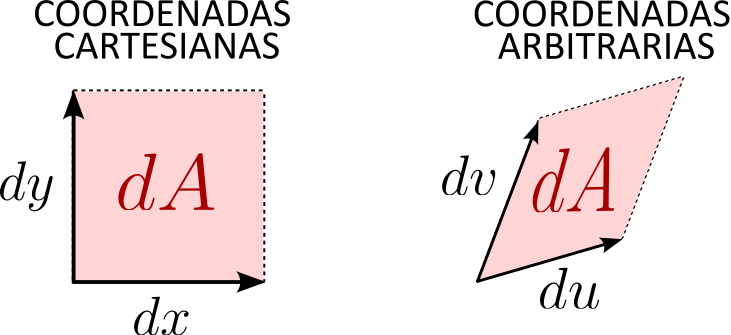
\includegraphics[scale=.4]{FOTOS/elem_area.png}
\end{center}
En el caso de las coordenadas cartesianas, el elemento diferencial de área se calculará como $\odif{A}=\odif{x}\odif{y}$. Cuando usemos coordenadas arbitrarias, veremos que necesitaremos un 'determinante' que transforme el elemento de área cartesiano.\\

Sea una superficie con una carta local,
\begin{align*}
    \mathbf{x}:U\subseteq\mathbb{R}^2&\longrightarrow V \cap S\\
                        (u^1,u^2)&\longmapsto \mathbf{x}(u^1,u^2);
\end{align*}
y $\Omega \subset U$ es un dominio cerrado de $U$. Bajo estas condiciones, el área de $\mathbf{x}(\Omega)=\Sigma$ es:\\
\begin{wrapfigure}{r}{0.3\textwidth}
    \centering
    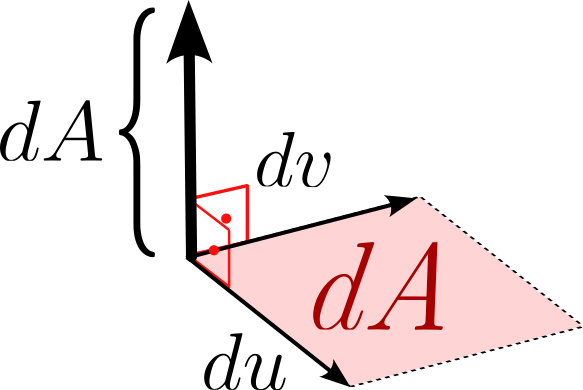
\includegraphics[scale=.3]{FOTOS/jacobiano.png}
\end{wrapfigure}
$$
A(\Sigma)=\int \!\!\!\!\int _\Omega \left | \left | \pdv{\mathbf{x}}{u^1}\wedge \pdv{\mathbf{x}}{u^2} \right | \right |\odif{u^1}\odif{u^2}
$$
En este caso, lo que actúa para modificar el elemento diferencial de área es el módulo del producto vectorial de los dos vectores de nuestra base de $T_p(S)$. Sustituyendo sus expresiones en el integrando, llegamos a que:
$$
A(\Sigma)=\int \!\!\!\!\int _\Omega ||\mathbf{x}_1\wedge \mathbf{x}_2||\odif{u^1}\odif{u^2}
$$

Ahora queda calcular el módulo de ese vector,
\begin{equation*}
    \begin{split}
        ||\mathbf{x}_1\wedge \mathbf{x}_2||^2&=(\mathbf{x}_1\wedge \mathbf{x}_2)\cdot (\mathbf{x}_1\wedge \mathbf{x}_2)\\
                                     &=||\mathbf{x}_1||^2||\mathbf{x}_2||^2 \sin ^2 \theta = ||\mathbf{x}_1||^2 ||\mathbf{x}_2||^2 (1-\cos ^2 \theta)\\
                                     &=g_{11}\cdot g_{22}(1-\cos ^2 \theta)=g_{11}g_{22}-g_{12}g_{21}\equiv g \ \left (=\det{g_{\alpha\beta}}\right )
    \end{split}
\end{equation*}
Y finalmente:
$$
\boxed{A(\Sigma)=\int \!\!\!\!\int _\Omega \sqrt{g}\odif{u^1}\odif{u^2}}
$$
\section{Vectores contravariantes y covariantes}
Ahora nos planteamos qué tipo de reparametrizaciones podemos usar.

Es importante recordar que las longitudes \emph{no cambian} bajo reparametrizaciones. El tensor métrico que hemos calculado servirá como regla de medida, e independientemente del convenio que usemos, estas longitudes siempre serán las mismas.
$$
t\xlongrightarrow{\text{difeomorf.}}\Bar{t}(t)
$$
\subsection{Reparametrizaciones}
Sea $\vec{\Phi}$ un difeomorfismo de $\Bar{U}$ en $U$:
\begin{align*}
    \vec{\Phi}:\Bar{U}\subseteq \mathbb{R}^2 &\longrightarrow U\subseteq \mathbb{R}^2\\
    (\Bar{u}^1,\Bar{u}^2)&\longmapsto \left ( \Bar{u}^1(u^1,u^2),\Bar{u}^2(u^1,u^2) \right )
\end{align*}

$\vec{\Phi}$ es un \emph{homeomorfismo} diferenciable, con función inversa diferenciable. Es decir, en la región de intersección entre dos cartas de una superficie, la función de transición tiene que ser un difeomorfismo. Se cumple por tanto que:
\begin{enumerate}
    \item[I)] $\vec{\Phi}:\Bar{U}\longrightarrow U$ es \emph{biyectiva}.
    \item[II)] $\vec{\Phi}:\Bar{U}\longrightarrow U$ es diferenciable ($\vec{\Phi}\in C^\infty$).
    \item[III)] $\vec{\Phi}^{-1}:U\longrightarrow \Bar{U}$ es diferenciable (de clase $C^\infty$).
\end{enumerate}

En notación más compacta, escribiremos el difeomorfismo como:
$$
\boxed{u^\alpha=u^\alpha (\Bar{u}^\beta)} \ , \ \text{con }\alpha,\beta=1,2
$$

El jacobiano de la \emph{transformación directa} es el determinante:
$$
D=\det{\left ( \pdv{u^\alpha}{\Bar{u}^\beta} \right )}
$$
y el de la \emph{transformación inversa} es:
$$
\Bar{D}=\det{\left ( \pdv{\Bar{u}^\alpha}{u^\beta} \right )} \ ;
$$
ambos con $\alpha,\beta=1,2$. Además, por el \emph{Teorema de la función inversa}, se cumple que:
$$
\pdv{u^\alpha}{\Bar{u}^\beta}\cdot \pdv{\Bar{u}^\beta}{u^\gamma }=\delta ^\alpha {}_\gamma  \xleftrightarrow{\text{matric.}} D\cdot \Bar{D}=\mathbb{1}
$$

\begin{mybox}
    \underline{Ejemplo C:} $u^1(\Bar{u}^1,\Bar{u}^2)=e^{\Bar{u}^1+\Bar{u}^2}\ , \ u^2(\Bar{u}^1,\Bar{u}^2)=e^{\Bar{u}^1-\Bar{u}^2}$\\

    $\hookrightarrow$ La transformación inversa es: $ \left \{
    \begin{array}{ccc}
         \Bar{u}^1&=&1/2\log(u^1\cdot u^2)  \\
         \Bar{u}^2&=&1/2\log(u^1/u^2) 
    \end{array} \right . \ \left (\Bar{u}^\alpha (u^\beta)\right )
    $\\
    $
    \rightarrow D^\alpha _\beta =\left ( \pdv{u^\alpha}{\Bar{u}^\beta} \right )=\left ( 
    \begin{array}{cc}
         e^{\Bar{u}^1+\Bar{u}^2}&e^{\Bar{u}^1+\Bar{u}^2}  \\
         e^{\Bar{u}^1-\Bar{u}^2}&-e^{\Bar{u}^1-\Bar{u}^2} 
    \end{array}
    \right ) = \left ( 
    \begin{array}{cc}
         u^1&u^1  \\
         u^2&-u^2 
    \end{array}
    \right )\implies D=-2u^1u^2
    $\\
    $
    \rightarrow \Bar{D}^\alpha_ \beta =\left ( \pdv{\Bar{u}^\alpha}{u^\beta} \right )= \cdots =\left ( 
    \begin{array}{cc}
         1/(2u^1)&1/(2u^2)  \\
         1/(2u^1)&-1/(2u^2) 
    \end{array}
    \right ) \implies \Bar{D}=-\frac{1}{2u^1u^2}
    $\\
    $
    \implies \left ( \pdv{u^\alpha}{\Bar{u}^\beta} \right ) \left ( \pdv{\Bar{u}^\alpha}{u^\beta} \right )=\delta ^\alpha {}_\beta  \qquad(D^\alpha _\beta \Bar{D}^\beta _\gamma =\delta ^\alpha {}_\gamma  )
    $
\end{mybox}

Veamos cómo se relacionan las bases en el plano tangente $T_p(S)$ tras una reparametrización.
$$
\Bar{\mathbf{x}}(\Bar{u}^1,\Bar{u}^2)=\mathbf{x}\left (u^1(\Bar{u}^1,\Bar{u}^2),u^2(\Bar{u}^1,\Bar{u}^2)\right )
$$
En notación compacta, diremos que $\Bar{\mathbf{x}}(\Bar{u}^\beta)=\mathbf{x}(u^\alpha (\Bar{u}^\beta))$. Cada carta $(U,\mathbf{x}(u^\alpha))$ y $(\Bar{U},\Bar{\mathbf{x}}(\Bar{u}^\beta))$ tiene un plano tangente, o más bien, una base de vectores del plano tangente $T_p(S)$.
$$
\left \{ \mathbf{x}_1=\pdv{\mathbf{x}}{u^1},\mathbf{x}_2=\pdv{\mathbf{x}}{u^2} \right \} \ , \ \left \{ \Bar{\mathbf{x}}_1=\pdv{\Bar{\mathbf{x}}}{\Bar{u}^1}, \Bar{\mathbf{x}}_2=\pdv{\Bar{\mathbf{x}}}{\Bar{u}^2} \right \}
$$

Busquemos la relación entre $\mathbf{x}_\alpha$ y $\mathbf{x}_\beta$. Por la regla de la cadena,
$$
\Bar{\mathbf{x}}_\beta = \pdv{\Bar{\mathbf{x}}}{\Bar{u}^\beta}=\pdv{\mathbf{x}}{u^\alpha}\cdot \pdv{u^\alpha}{\Bar{u}^\beta}=\pdv{u^\alpha}{\Bar{u}^\beta}\cdot \pdv{\mathbf{x}}{u^\alpha}=\pdv{u^\alpha}{\Bar{u}^\beta}\mathbf{x}_\alpha
$$
Es decir:
$$
\boxed{\Bar{\mathbf{x}}_\beta =\pdv{u^\alpha}{\Bar{u}^\beta}\mathbf{x}_\alpha}
$$

Esta es la relación entre las bases $\{ \mathbf{x}_\alpha  \}$ y $\{ \Bar{\mathbf{x}}_\beta \}$ tras el cambio de coordenadas. $\left ( \pdv{u^\alpha}{\Bar{u}^\beta} \right )$ es la \emph{matriz de cambio de base}. Su transformación inversa es:
$$
\boxed{\mathbf{x}_\alpha=\pdv{\Bar{u}^\beta}{u^\alpha}\Bar{\mathbf{x}}_\beta}
$$
\begin{mybox}
    \begin{center}
        \textbf{ORIENTABILIDAD}
    \end{center}
    Para que las cartas $(U,\mathbf{x}(u^\alpha))$ y $(\Bar{U},\Bar{\mathbf{x}}(\Bar{u}^\beta))$ describan la misma superficie y den lugar al mismo plano tangente (con el vector perpendicular en la misma orientación), se tiene que cumplir que
    $$
    D=\det{\pdv{u^\alpha}{\Bar{u}^\beta}}>0
    $$
    Si no lo cumple, hacemos el cambio $\Bar{u}^1\leftrightarrow \Bar{u}^2$.
\end{mybox}

Resumiendo, bajo difeomorfismos, tenemos las siguientes \emph{reglas de cambio de base}.
\begin{mybox}
    \begin{center}
        \textbf{CAMBIO DE BASE}
    \end{center}
    Bajo difeomorfismos (por la regla de la cadena), tenemos que, en las bases $\{\mathbf{x}_\alpha\}$ y $\{ \Bar{\mathbf{x}}_\beta \}$.
    $$
    \mathbf{x}_\alpha=\pdv{\Bar{u}^\beta}{u^\alpha}\Bar{\mathbf{x}}_\beta \qquad  \qquad \Bar{\mathbf{x}}_\beta=\pdv{u^\alpha}{\Bar{u}^\beta}\mathbf{x}_\alpha
    $$
\end{mybox}

\subsection{Leyes de transformación}
Sea $\mathbf{v}\in T_p(S)$. Entonces, $\mathbf{v}=v^\alpha \mathbf{x}_\alpha$ (con el convenio de Einstein), o bien, si decidimos transformarlo a otras coordenadas, $\mathbf{v}=\Bar{v}^\alpha \Bar{\mathbf{x}}_\alpha$. $v^\alpha$ y $\Bar{v}^\alpha$ son las componentes del vector entre las bases $\{ \mathbf{x}_\alpha \}$ y $\{ \Bar{\mathbf{x}}_\alpha \}$. Usando la información del cambio de base visto anteriormente, decimos que:
\begin{gather*}
    \mathbf{v}=v^\alpha \mathbf{x}_\alpha =v^\alpha \pdv{\Bar{u}^\beta}{u^\alpha} \Bar{\mathbf{x}}_\beta=\Bar{v}^\beta \Bar{\mathbf{x}}_\beta \\
    \boxed{\Bar{v}^\beta=\pdv{\Bar{u}^\beta}{u^\alpha}v^\alpha}
\end{gather*}
Esta es la \emph{ley de transformación de las componentes contravariantes} de un vector (veremos más adelante por qué las llamaremos contravariantes). De hecho, las relaciones de cambio de base serán las leyes de transformación de los vectores covariantes de la base en $T_p(S)$.\\

\begin{wrapfigure}{l}{.4\textwidth}
    \centering
    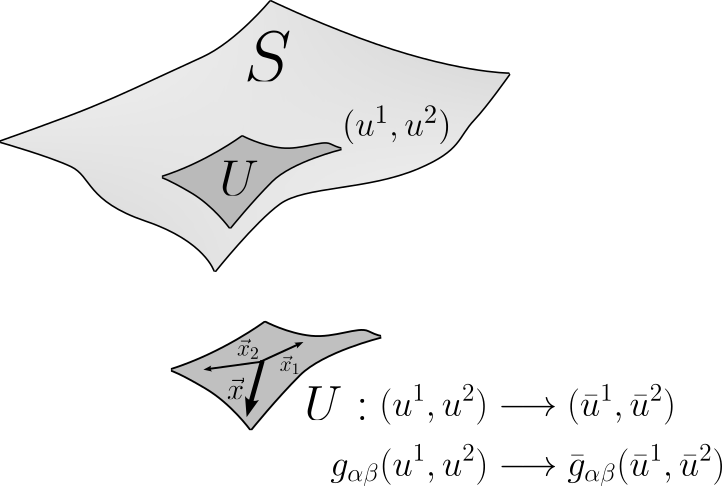
\includegraphics[scale=.45]{FOTOS/forma_fundamental_trans.png}
\end{wrapfigure}

Veamos ahora cuál es la regla de transformación de la primera forma fundamental bajo reparametrizaciones (con difeomorfismos).
\begin{align*}
    g_{\alpha \beta}      =\mathbf{x}_\alpha \cdot \mathbf{x}_\beta \longrightarrow    
    \Bar{g}_{\alpha \beta}&=\Bar{\mathbf{x}}_\alpha \cdot \Bar{\mathbf{x}}_\beta\\
                          &=\left ( \pdv{u^\mu}{\bar{u}^\alpha}\mathbf{x}_\mu  \right ) \cdot \left ( \pdv{u^\nu}{\bar{u}^\beta}\mathbf{x}_\nu  \right )\\
                          &=\pdv{u^\mu}{\bar{u}^\alpha} \pdv{u^\nu}{\bar{u}^\beta} \mathbf{x}_\mu \cdot \mathbf{x}_\nu\\
                          &=\pdv{u^\mu}{\bar{u}^\alpha} \pdv{u^\nu}{\bar{u}^\beta} g_{\mu \nu}
\end{align*}
$$
\boxed{\Bar{g}_{\alpha \beta}=\pdv{u^\mu}{\bar{u}^\alpha} \pdv{u^\nu}{\bar{u}^\beta} g_{\mu \nu}}
$$
\WFclear
\begin{itemize}
    \item \emph{Comentario}: Los índices $\alpha,\beta,\mu,\nu$ que aparecen \emph{abajo} son índices \emph{covariantes.} 
\end{itemize}

Bajo difeomorfismos, el determinante de la primera forma fundamental se transforma según la siguiente ley:
\begin{equation*}
    \begin{split}
        g&=\det{g_{\alpha \beta}} =g_{11}g_{22}-g_{12}g_{21}\\
\implies   \Bar{g}&=\Bar{g}_{11}\Bar{g}_{22}-\Bar{g}_{12}\Bar{g}_{21} \\
& =\left ( \pdv{u^\mu}{\bar{u}^1} \pdv{u^\nu}{\bar{u}^1} \right )g_{\mu \nu}\cdot \left ( \pdv{u^\rho}{\bar{u}^2} \pdv{u^\sigma}{\bar{u}^2} \right )g_{\rho \sigma} - \left ( \pdv{u^\mu}{\bar{u}^1} \pdv{u^\nu}{\bar{u}^2} \right )g_{\mu \nu}\cdot \left ( \pdv{u^\rho}{\bar{u}^2} \pdv{u^\sigma}{\bar{u}^1} \right )g_{\rho \sigma} \\
         &=g\cdot D^2 \quad , \quad \text{con $D$ el determinante jacobiano}
    \end{split}
\end{equation*}
$$
\boxed{\Bar{g}=gD^2}
$$

Y, por lo tanto, la ley de transformación de $g$ asegura que el área de una superficie sea invariante bajo reparametrizaciones por un difeomorfismo.
\begin{align*}
    A(\Sigma)      &=\int \! \! \! \! \int _\Omega \sqrt{g}\odif{u^1}\odif{u^2}\\
    \Bar{A}(\Sigma)&=\int \! \! \! \! \int _{\Bar{\Omega}} \sqrt{\Bar{g}} \odif{\Bar{u}^1} \odif{\Bar{u}^2} =\int \! \! \! \! \int _\Omega \sqrt{D^2 g}\ |\Bar{D}|\odif{u^1}\odif{u^2}=\int \! \! \! \! \int _\Omega \sqrt{g}\odif{u^1}\odif{u^2}=A(\Sigma) \ \smiley
\end{align*}

\subsection{Base dual. Componentes covariantes de un vector}
Dado el plano tangente a la superficie $T_p(S)$, una base de dicho plano es $\left \{ \mathbf{x}_1=\pdv{\mathbf{x}}{u^1},\mathbf{x}_2=\pdv{\mathbf{x}}{u^2} \right \}\equiv B$. Una base del espacio vectorial \emph{dual} a $T_p(S)$, $T_p^*(S)$, será:
$$
\left \{ \mathbf{x}^{1*},\mathbf{x}^{2*} \right \}=\left \{ \mathbf{x}^1,\mathbf{x}^2 \right \}.
$$

En esta base, los vectores tienen \emph{superíndices} en vez de subíndices. y cumplen que:
$$
\mathbf{x}^\alpha \cdot \mathbf{x}_\beta =\delta ^\alpha {}_\beta 
$$

\begin{mybox}
    \underline{Ejemplo D:} En $\mathbb{R}^2$, $\left \{ \mathbf{x}_1=(2,0),\mathbf{x}_2=\left ( \frac{1}{\sqrt{2}},\frac{1}{\sqrt{2}} \right ) \right \}$. La base dual debe cumplir que:
    \begin{itemize}
        \item $\mathbf{x}^2$ debe ser ortogonal a $\mathbf{x}_1$ y paralelo a $\mathbf{x}_2$.\\
        $\implies \mathbf{x}^2$ es de la forma $\mathbf{x}^2=(0,a) \ (\mathbf{x}^2\cdot \mathbf{x}_1=0)$\\
        $\implies a=\sqrt{2}$ (por la condición $\mathbf{x}^2\cdot \mathbf{x}_2=1$)
        $$
        \iff \mathbf{x}^2=\left (0,\sqrt{2} \right )
        $$

        \item $\mathbf{x}^1$ debe ser ortogonal a $\mathbf{x}_2$ y paralelo a $\mathbf{x}_1$.\\
        $\implies \mathbf{x}^1=(b,-b)$ ($\mathbf{x}^1\cdot \mathbf{x}_2=0$)\\
        $\implies b=1/2$ ($\mathbf{x}^1\cdot \mathbf{x}_1=1$)
        $$
        \iff \mathbf{x}^1=\left ( \frac{1}{2},-\frac{1}{2} \right )
        $$
    \end{itemize}
    $$
    B^*=\left \{ \mathbf{x}^1=\left ( \frac{1}{2},-\frac{1}{2} \right ),\mathbf{x}^2=\left (0,\sqrt{2} \right ) \right \}
    $$
    que es una base de $\left (\mathbb{R}^2\right )^*=\mathbb{R}^2$ (espacios auto-duales).
\end{mybox}
La idea de introducir la base dual es para poder calcular las componentes \emph{contravariantes} de un vector mediante productos escalares. Supongamos que tenemos $\mathbf{v}\in T_p(S)$, $\left \{ \mathbf{x}_\alpha \right \}$ una base de ese espacio y $\{ \mathbf{x}^\beta  \}$ del espacio dual.
\begin{gather*}
    \mathbf{v}=v^\alpha \mathbf{x}_\alpha \\
    \mathbf{v} \cdot \mathbf{x}^\beta=(v^\alpha \mathbf{x}_\alpha) \cdot \mathbf{x}^\beta =v^\alpha (\mathbf{x}_\alpha \cdot \mathbf{x}^\beta)=v^\alpha \delta _\alpha {}^\beta =v^\beta
\end{gather*}
$$
\boxed{\mathbf{v}\cdot \mathbf{x}^\beta=v^\beta}
$$
Veamos ahora la relación entre las bases $B$ y $B^*$. Definiremos para eso la inversa de la primera forma fundamental como:
$$
g_{\alpha \beta }^{-1}=g^{\alpha \beta } \qquad \qquad \text{como matrices, }g_{\alpha \beta} \cdot g^{\beta \gamma}=\delta ^\gamma {}_\alpha
$$

Los vectores de esta base dual $B^*$, $\{ \mathbf{x}^\alpha \}$ cumplen entonces que 
\begin{equation*}
    \begin{split}
        \mathbf{x}^\alpha=g^{\alpha \beta} \mathbf{x}_\beta \longrightarrow \mathbf{x}^\alpha \cdot \mathbf{x}_\beta &=g^{\alpha \beta}\mathbf{x}_\rho \cdot \mathbf{x}_\beta\\
        &=g^{\alpha \rho}g_{\rho \beta} =\delta ^\alpha {}_\beta 
    \end{split}
\end{equation*}

Las componentes de un vector en la base dual $B^*$ se denominan, por tanto, \emph{componentes covariantes} del vector, y se tiene que 
$$
\mathbf{v}=v^\alpha \mathbf{x}_\alpha =v_\beta \mathbf{x}^\beta =v_\beta g^{\alpha \rho}\mathbf{x}_\rho 
$$
$$
\boxed{v^\alpha =v_\beta g^{\beta \alpha} =g^{\alpha\beta}v_\beta}
$$
Es decir, $g^{\alpha \beta}$ permite subir índices. De forma análoga, $g_{\alpha \beta}$ permite bajar índices,
$$
v_\alpha =g_{\alpha \beta} v^\beta
$$
\begin{mybox}
    \begin{center}
        \textbf{COMPONENTES COVARIANTES Y CONTRAVARIANTES}
    \end{center}
    Las componentes \textbf{contravariantes} de $\mathbf{v}$ son $v^\alpha$. Las componentes \textbf{covariantes} de $\mathbf{v}$ son $v_\alpha$. Por convenio, usamos la notación \emph{covariante} para denotar \emph{subíndices}; y \emph{contravariante} para denotar \emph{superíndices}. La relación entre componentes covariantes y contravariantes es:
    \begin{gather*}
        v^\alpha=g^{\alpha\beta}v_\beta \qquad \qquad v_\alpha =g_{\alpha \beta} v^\beta
    \end{gather*}
    con $g^{\alpha \beta }=g_{\alpha \beta }^{-1} $ la inversa de la primera forma fundamental.
\end{mybox}
Los nombres se deben a la manera en la que se transforman bajo cambios de coordenadas o difeomorfismos.\\

Sea $u^\alpha =u^\alpha (\Bar{u}^\beta)$ el cambio de coordenadas. Por la regla de la cadena:
$$
\Bar{\mathbf{x}}_\alpha =\pdv{u^\beta }{\Bar{u}^\alpha }\mathbf{x}_\beta 
$$
$
\implies
$ Los vectores covariantes se transforman con la matriz $\pdv{u^\beta }{\Bar{u}^\alpha}$

Las componentes contravariantes $\Bar{v}^\alpha =\pdv{\Bar{u}^\alpha }{u^\beta }v^\beta$ se transforman con la matriz inversa.
$$
\underbrace{\pdv{u^\beta }{\Bar{u}^\alpha }}_{\text{\parbox{4cm}{\centering
Matriz directa\\ Prefijo 'co'}}} \qquad  \underbrace{\pdv{\Bar{u}^\alpha }{u^\beta}}_{\text{\parbox{4cm}{\centering
Matriz inversa\\ Prefijo 'contra'}}}
$$

Las componentes covariantes se transforman con la primera forma fundamental transformada, $\Bar{g}_{\alpha \beta}$, como sigue:
\begin{equation*}
    \begin{split}
        \Bar{v}_\alpha=\Bar{g}_{\alpha \beta} \Bar{v}^\beta &=\pdv{u^\rho }{\Bar{u}^\alpha }\pdv{u^\sigma }{\Bar{u}^\beta }g_{\rho \sigma} \Bar{v}^\beta=\pdv{u^\rho }{\Bar{u}^\alpha }\pdv{u^\sigma }{\Bar{u}^\beta}g_{\rho \sigma }\pdv{\Bar{u}^\beta }{u^\gamma }v^\gamma\\
        &= \pdv{u^\rho }{\Bar{u}^\alpha }\delta ^\sigma{}_\gamma  g_{\rho \sigma }v^\gamma =\pdv{u^\rho }{\Bar{u}^\alpha } v_\rho =\pdv{u^\beta }{\Bar{u}^\alpha }v_\beta
    \end{split}
\end{equation*}
$$
\boxed{\Bar{v}_\alpha =\pdv{u^\beta }{\Bar{u}^\alpha }v_\beta}
$$
\begin{mybox}
    \begin{center}
        \textbf{LEYES DE TRANSFORMACIÓN DE COMPONENTES}
    \end{center}
    $$
    \begin{array}{ccc}
         \text{\textbf{Matriz directa}}&& \text{\textbf{Matriz inversa}} \\
         \cfrac{\partial u^\beta }{\partial \Bar{u}^\alpha }&&\cfrac{\partial \Bar{u}^\alpha }{\partial u^\beta}\\
         \Bar{v}_\alpha =\cfrac{\partial u^\beta }{\partial \Bar{u}^\alpha }v_\beta&&\Bar{v}^\alpha =\cfrac{\partial \Bar{u}^\alpha }{\partial u^\beta }v^\beta 
    \end{array} 
    $$
\end{mybox}

En $T_p(S)$ tenemos un producto escalar. Si $\mathbf{v},\mathbf{w}\in T_p(S)$, entonces:
\begin{equation*}
    \begin{split}
        \left . \begin{array}{ccc}
             \mathbf{v}&=&v^\alpha \mathbf{x}_\alpha   \\
             \mathbf{w}&=&w^\beta \mathbf{x}_\beta  
        \end{array} \right \} \longrightarrow \mathbf{v}\cdot \mathbf{w}&=v^\alpha w^\beta \mathbf{x}_\alpha \mathbf{x}_\beta =v^\alpha w^\beta g_{\alpha \beta}\\
        &=v_\beta w^\beta =v^\alpha w_\alpha 
    \end{split}
\end{equation*}

La contracción de los índices covariantes y contravariantes de las componentes de un vector da lugar a una cantidad \emph{escalar} (que más adelante veremos que es invariante).

\subsection{Tensores}
El cambio de índices o componentes covariantes a contravariantes y viceversa se lleva a cabo mediante la inversa de la primera forma fundamental, o mediante la propia primera forma fundamental. \\

$\rightarrow $ BAJAR ÍNDICES: Contravariante $\to $ covariante\\
$$
v_\alpha =g_{\alpha \beta }v^\beta
$$

$\rightarrow $ SUBIR ÍNDICES: Covariante $\to $ contravariante\\
$$
v^\alpha =g^{\alpha \beta} v_\beta 
$$

La primera forma fundamental $g_{\alpha \beta} =\mathbf{x}_\alpha \cdot \mathbf{x}_\beta $ con dos índices no repetidos (o libres) es un ejemplo de \emph{tensor} de segundo orden.
\begin{itemize}
    \item El número de índices del tensor indica su \emph{orden tensorial}.
    \item Si los índices están \emph{abajo}, como $g_{\alpha \beta}$, el tensor se dice \emph{dos veces covariante}.
    
    $\hookrightarrow$Covariante dos veces: $ \Bar{g}_{\alpha \beta} = \pdv{u^\mu }{\Bar{u}^\alpha }\pdv{u^\nu }{\Bar{u}^\beta }g_{\mu \nu}$ 
    \item Si los índices están \emph{arriba}, como $g^{\alpha \beta} $, el tensor se dice \emph{dos veces contravariante}.
    
    $\hookrightarrow $Contravariante dos veces: $\Bar{g}^{\alpha \beta}=\pdv{\Bar{u}^\alpha }{u^\mu }\pdv{\Bar{u}^\beta }{u^\nu }g^{\mu \nu}$

    \item Cuando un tensor tiene tanto índices covariantes como índices contravariantes, se conoce como tensor \emph{mixto} (que puede ser $k$ veces covariante y $j$ veces contravariante).\\

    $\hookrightarrow$ Para la primera forma fundamental:
    $$
    \Bar{g}^\alpha{} _\beta=\pdv{\Bar{u}^\alpha }{u^\mu} \pdv{u^\nu }{\Bar{u}^\beta }g^\mu {}_\nu \longrightarrow g^\mu{} _\nu =g^{\mu \rho }g_{\rho \nu }=\delta ^\mu{}_\nu 
    $$

    \item Los tensores con más de dos índices son tensores de orden superior.
\end{itemize}
\section{Geometría riemanniana}
La geometría riemanniana extiende la noción de superficie a lo que se conoce como \emph{variedades} de dimensión $n$ (las superficies son variedades bidimensionales). Localmente, en una variedad diferenciable de dimensión $n$, podemos introducir un sistema de coordenadas $(u^1,u^2,\ldots , u^n)$ y un conjunto de $n^2$ funciones $g_{\alpha \beta} (u^1,u^2,\ldots, u^n)$, donde $\alpha ,\beta=1,2,\ldots , n$, y ordenadas matricialmente; que cumplen lo siguiente:
\begin{enumerate}
    \item[I)] La matriz es simétrica, $g_{\alpha \beta}=g_{\beta \alpha}$
    \item[II)] La matriz es definida positiva, es decir, todos sus menores son positivos.
    \item[III)] Al cambiar de carta por una reparametrización,
    $$
    \Bar{g}_{\alpha \beta}=\pdv{u^\mu }{\Bar{u}^\alpha }\pdv{u^\nu }{\Bar{u}^\beta }g_{\mu \nu}
    $$
\end{enumerate}
(El segundo requerimiento puede no cumplirse en el caso de encontrarnos en geometría pseudo-riemanniana, como en Relatividad General.)\\

En geometría riemanniana, las funciones $g_{\alpha \beta} $ se conocen como \emph{métrica} o \emph{tensor métrico}.
\begin{gather*}
    \odif{S^2}=g_{\alpha \beta} \odif{u^\alpha}\odif{u^\beta}\\
    \alpha ,\beta =1,2,\ldots, n
\end{gather*}

Para el caso en el que la dimensión $n=2$, recuperamos las variedades o superficies bidimensionales. De forma general, el tensor métrico $g_{\alpha \beta}$ representa el \emph{elemento de línea} de la variedad, $\odif{S^2}=g_{\alpha \beta} \odif{u^\alpha }\odif{u^\beta}$.

\begin{wrapfigure}{r}{.37\textwidth}
    \centering
    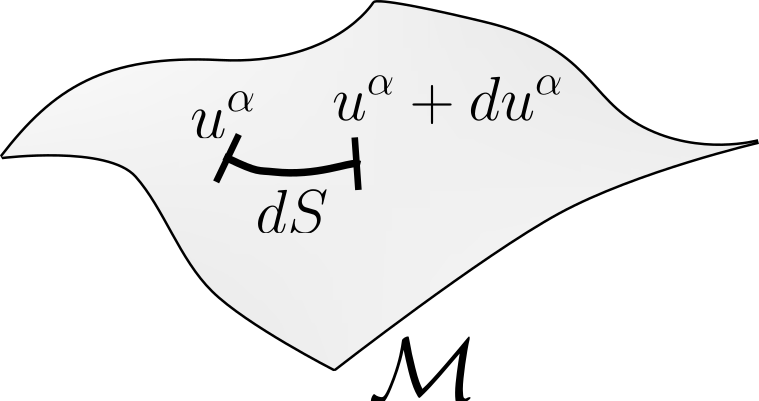
\includegraphics[scale=.3]{FOTOS/manifold.png}
\end{wrapfigure}

Dada la variedad $\mathcal{M}$ de dimensión $n$, para construir el espacio $T_p(\mathcal{M})$, de dimensión $n$, necesitamos las derivadas direccionales $\mathbf{x}_\alpha $, con $\alpha =1,2,\ldots ,n$. 

En el caso de las superficies bidimensionales conocemos $\mathbf{x}(u^1,u^2)$, esto es, la carta local de la superficie $S$. En general, para variedades $\mathcal{M}$ no se conoce $\mathbf{x}(u^1,\ldots , u^n)$.\\

Como no disponemos de $\mathbf{x}$, lo eliminaremos de la definición de las derivadas direccionales.
$$
\mathbf{x}_\alpha =\left .\pdv{}{u^\alpha }\right |_{(u^1,u^2,\ldots,u^n)}
$$
De este modo: $\mathbf{v}\in T_p(\mathcal{M}) \ , \ \mathbf{v}=v^\alpha \mathbf{x}_\alpha =v^\alpha \partial _\alpha $ con $\alpha =1,\ldots ,n$ y $\partial_\alpha =\pdv{}{u^\alpha }$.\\

Con esta definición, $v^\alpha $ son las componentes contravariantes del vector $\mathbf{v}\in T_p(\mathcal{M})$. Para verlo, basta con cambiar de parametrización en $\mathcal{M}$, $(\Bar{u}^1,\Bar{u}^2,\ldots ,\Bar{u}^n)\longrightarrow (u^1,u^2,\ldots , u^n)$.
\begin{align*}
    \mathbf{v}&=v^\alpha \mathbf{x}_\alpha =v^\alpha \partial_\alpha =v^\alpha \pdv{}{u^\alpha }\\
    \downarrow&\\
    \Bar{\mathbf{v}}&=\Bar{v}^\beta \Bar{\mathbf{x}}_\beta =\Bar{v}^\beta \Bar{\partial}_\beta =\Bar{v}^\beta \pdv{}{\Bar{u}^\beta }
\end{align*}
Como $\mathbf{v}=\Bar{\mathbf{v}}$:
\begin{gather*}
    v^\alpha \partial_\alpha =v^\alpha \pdv{}{u^\alpha }=v^\alpha \pdv{\Bar{u}^\beta }{u^\alpha }\pdv{}{\Bar{u}^\beta }=\pdv{\Bar{u}^\beta }{u^\alpha } v^\alpha \Bar{\partial}_\beta \\
    \boxed{\Bar{v}^\beta =\pdv{\Bar{u}^\beta }{u^\alpha } v^\alpha }
\end{gather*}
que es la ley de transformación de las componentes contravariantes de $\mathbf{v}$. \\

Para una variedad $\mathcal{M}$ de dimensión $n$, la base dual del espacio tangente, $\{ \mathbf{x}^\alpha  \}$, se construye a través del producto interno (o escalar) definido en $T_p(\mathcal{M})$. Para asegurar que se cumple que $\langle \mathbf{x}^\alpha , \mathbf{x}_\beta \rangle =\delta ^\alpha {}_\beta  $ (el producto que define el espacio vectorial dual), basta con tomar los $\mathbf{x}^\alpha $ como:
$$
\boxed{\mathbf{x}^\alpha =\odif{u^\alpha }} \ ,
$$
que son los diferenciales de línea, conocidos también como 1-formas diferenciables de Cartan. Los elementos de la base dual, $\{ \odif{u^\alpha } \}$, cumplen que:
$$
\Bar{\mathbf{x}}^\alpha =\odif{\Bar{u}^\alpha }=\pdv{\Bar{u}^\alpha }{u^\beta }\odif{u^\beta} =\pdv{\Bar{u}^\alpha }{u^\beta } \mathbf{x}^\beta \ ,
$$
que es la ley de transformación contravariante.
\begin{mybox}
    $\left \{ \begin{array}{cccc}
        \mathbf{x}_\alpha  &=&\partial_\alpha&  \\
        &&&\text{con }\alpha =1,\ldots ,n\\
         \mathbf{x}^\alpha &=&\odif{u^\alpha }&
    \end{array} \right | \ \text{\parbox{8cm}{El espacio dual a $T_p(\mathcal{M})$, cuya base es $\{ \mathbf{x}^\alpha  \}=\{ \odif{u^\alpha } \}$, se conoce como el espacio \textbf{cotangente} a $\mathcal{M}$ en el punto $P$.}}$ 
\end{mybox}

De esta forma, para la variedad $\mathcal{M}$, el producto escalar en $T_p(\mathcal{M})$ está definido como:
\begin{equation*}
    \begin{split}
        \begin{array}{c}
             \mathbf{v}=v^\alpha \mathbf{x}_\alpha   \\
             \mathbf{w}=w^\beta \mathbf{w}_\beta
        \end{array} \ ; \ \mathbf{v},\mathbf{w}\in T_p(\mathcal{M}):\mathbf{v}\cdot \mathbf{w}&=v_\alpha w^\alpha =v^\beta w_\beta =g_{\alpha \beta }v^\alpha w^\beta\\
        \mathbf{v}&=v^\alpha \mathbf{x}_\alpha =v_\alpha \mathbf{x}^\alpha \\
      \text{Donde hemos usado}\quad   \mathbf{w}&=w^\beta \mathbf{x}_\beta =w_\beta \mathbf{x}^\beta \\
        v_\alpha &=g_{\alpha \beta }v^\beta \ \text{(subir y bajar índices)}
    \end{split}
\end{equation*}

El espacio de 1-formas en el espacio cotangente y las derivadas direccionales en el espacio tangente permiten construir tensores como aplicaciones, en base a su regla o ley de transformación. \\
De acuerdo con su ley de transformación, podemos clasificar los tensores de la siguiente manera:

\begin{enumerate}
    \item[(i)] \underline{Escalares:} Una aplicación es un escalar si $h=\Bar{h}$. Explícitamente:
    $$
    \Bar{h}(\Bar{u}^\alpha )=h(u^\alpha)
    $$
    Un escalar es una cantidad puramente geométrica e invariante frente al sistema de coordenadas elegido.

    \item[(ii)] \underline{Vectores o tensores de orden uno:} \\
    En componentes contravariantes$\longrightarrow \Bar{v}^\beta =\pdv{\Bar{u}^\beta }{u^\alpha }v^\alpha $\\
    En componentes covariantes    $\longrightarrow \Bar{u}_\beta =\pdv{u^\beta }{\Bar{u}^\alpha }v_\alpha $\\

    \item[(iii)] \underline{Tensores de orden dos:} \\
    Dos veces contravariante $\longrightarrow \Bar{a}^{\alpha \beta} =\pdv{\Bar{u}^\alpha }{u^\mu }\pdv{\Bar{u}^\beta }{u^\nu}a^{\mu \nu}$\\
    Dos veces covariantes$\longrightarrow \Bar{a}_{\alpha \beta} =\pdv{u^\mu}{\Bar{u}^\alpha }\pdv{u^\nu }{\Bar{u}^\beta }a_{\mu \nu}$\\
    Tensor mixto (1 covariante 1 contravariante)$\longrightarrow \Bar{a}^\alpha {}_\beta =\pdv{\Bar{u}^\alpha }{u^\mu }\pdv{u^\nu }{\Bar{u}^\beta }a^\mu {}_\nu $

    \item[(iv)] \underline{Tensor de orden $r+s$ (r veces covariante, s veces contravariante)}:
    $$
    \Bar{h}_{\alpha _1,\ldots ,\alpha _r}{}^{\beta_1,\ldots ,\beta_s}=\pdv{u^{\mu_1}}{\Bar{u}^{\alpha _1}}\cdots \pdv{u^{\mu_r}}{\Bar{u}^{\alpha _r}}\pdv{\Bar{u}^{\beta _1}}{u^{\nu_1}}\cdots \pdv{\Bar{u}^{\beta _s}}{u^{\nu_s}} h_{\mu_1,\ldots , \mu _r}{}^{\nu_1, \ldots , \nu_s} 
    $$
\end{enumerate}
\section{Fundamentos del cálculo tensorial}
\begin{itemize}
   \item La \emph{suma} de tensores está definida para tensores del mismo tipo (con la misma disposición de índices).

    Por ejemplo: $a^\mu {}_\nu +b^\mu {}_\nu =c^\mu {}_\nu $.\\

   \item El \emph{producto tensorial} está definido para tensores de cualquier tipo.

    Por ejemplo: $a^\mu {}_\nu b^\rho =c^\mu {}_\nu {}^\rho \longrightarrow \text{\parbox{7.5cm}{Tensor de orden tres, dos veces contravariante, una vez covariante.}}$

    \item La \emph{contracción de índices} reduce el orden del tensor.

    Dado $a^\mu {}_\nu:\ a^\mu {}_\nu \longrightarrow a^\mu {}_\mu =a^1{}_1+a^2{}_2+\ldots +a^n{}_n$, que es un escalar.\\

    La contracción de índices en un tensor mixto de orden 2 es la traza de la matriz asociada a dicho tensor.
    $$
    R^\mu {}_{\nu \rho \sigma }\xlongrightarrow{\mu =\rho } R^\mu {}_{\nu \mu \sigma }=R_{\nu \sigma }
    $$
    (la contracción en $R^\mu {}_{\nu \rho \sigma}$, que es el tensor de Riemann, da lugar al tensor de Ricci).

    \item La bajada y subida de índices puede llevarse a cabo mediante el tensor métrico $g_{\mu \nu}$ y su inverso, $g^{\mu \nu}$.
\end{itemize}

Además, un tensor se dice \emph{simétrico} cuando, al intercambiar los índices, permanece invariante ($g_{\mu \nu}=g_{\nu \mu}$). Por el contrario, un tensor se dice antisimétrico cuando, al intercambiar dos índices, cambia de signo: $a_{\mu \nu}=-a_{\nu \mu}$.
\section{Tensores especiales}
La \emph{delta de Kronecker}, definida como $\delta _\alpha {}^\beta= \left \{ 
\begin{array}{ccc}
     1&,&\alpha =\beta   \\
     0&,&\alpha \neq \beta  
\end{array}  \right .$, es válida para cualquier sistema de coordenadas. Veamos cómo se transforma bajo cambios de coordenadas.
$$
\Bar{\delta }_\alpha {}^\beta =\pdv{\Bar{u}^\beta }{u^\mu }\pdv{u^\nu }{\Bar{u}^\alpha }\delta ^\mu {}_\nu =\frac{\partial \Bar{u}^\beta}{\cancel{\partial u^\mu}}\frac{\cancel{\partial u^\mu}}{\partial \Bar{u}^\alpha}=\delta _\alpha {}^\beta 
$$
Se trata de un tensor mixto, que no cambia bajo transformaciones de coordenadas.\\

No obstante, no todo aquello que tiene índices se comporta como un tensor. Por ejemplo, la cantidad conocida como el \emph{símbolo de Levi-Civita}, definido como:
$$
\epsilon_{\alpha \beta}=\left \{ 
\begin{array}{cccc}
     0&\text{si}&\alpha =\beta=1 \text{ ó } 2 & \\
     1&\text{si}&\alpha =1,\ \beta=2& \text{(permutación par)}  \\
     -1&\text{si}&\alpha =2,\ \beta=1& \text{(permutación impar)}
\end{array}
\right .
$$

La definición de $\epsilon_{\alpha \beta}$ no depende del sistema de coordenadas. Veamos si es un tensor (invariante). Como se da que si $\alpha =\beta ,\ \epsilon_{\alpha \beta}=0$; solo hay que comprobar los casos de $\epsilon _{12}$ y $\epsilon_{21}$.
\begin{itemize}
    \item[$\rightarrow$] $\mu =1,\ \nu=2$:
    $$
    \Bar{\epsilon}_{12}=\Bar{\epsilon }_{\alpha \beta }\pdv{u^\alpha }{\Bar{u}^1}\pdv{u^\beta }{\Bar{u}^2}=\overbrace{\epsilon_{12}}^{1}\pdv{u^1 }{\Bar{u}^1}\pdv{u^2 }{\Bar{u}^2}+\overbrace{\epsilon_{21}}^{-1}\pdv{u^2 }{\Bar{u}^1}\pdv{u^1 }{\Bar{u}^2}=D
    $$
    donde $D$ es el determinante jacobiano de la transformación.

    \item[$\rightarrow $]$\mu=2,\ \nu=1$:
    $$
    \Bar{\epsilon }_{21}=\Bar{\epsilon }_{\alpha \beta }\pdv{u^\alpha }{\Bar{u}^2}\pdv{u^\beta }{\Bar{u}^1}=\pdv{u^1 }{\Bar{u}^2}\pdv{u^2 }{\Bar{u}^1}-\pdv{u^2 }{\Bar{u}^2}\pdv{u^1 }{\Bar{u}^1}=-D
    $$
\end{itemize}

Finalmente, lo que vemos es que:
$$
\Bar{\epsilon }_{\mu \nu}=\pdv{u^\alpha }{\Bar{u}^\mu }\pdv{u^\beta }{\Bar{u}^\nu}\epsilon_{\alpha \beta}=D\epsilon_{\mu \nu}
$$
En este caso, no vemos que $\epsilon_{\mu \nu}\leftrightarrow\Bar{\epsilon }_{\mu \nu}\implies \epsilon_{\alpha \beta }$ \textbf{no} es invariante. Es decir, no se trata de un tensor. Si recordamos que $\Bar{g}=D^2g$,
$$
|D|=\sqrt{\Bar{g}/g}
$$
Las cantidades $\sqrt{g}\epsilon_{\alpha \beta}$ sí son invariantes (de acuerdo con las leyes de transformación), y se transforman como un tensor de segundo orden.
\begin{mybox}
    \begin{center}
        \textbf{TENSOR DE LEVI-CIVITA}
    \end{center}
    El tensor definido como:
    $$
    \varepsilon_{\alpha \beta }=\sqrt{g}\epsilon_{\alpha \beta}
    $$
    se transforma de acuerdo con las leyes de transformación de tensores. Esta cantidad se conoce como \textbf{pseudo-tensor de Levi-Civita}. Si la transformación de coordenadas cambia la orientación ($D<0$), la regla de transformación tiene un signo negativo global.
\end{mybox}

En dimensión $n$ se define el pseudo-tensor (o símbolo) de Levi-Civita como:
$$
\begin{array}{cccc}
     \epsilon_{\mu_1,\ldots , \mu_n}&=&0&\text{\parbox{8cm}{si hay dos índices repetidos}}  \\\\
     \epsilon_{\mu_1,\ldots , \mu_n}&=&1&\text{\parbox{8cm}{si $(\mu_1,\ldots , \mu_n)$ es una permutación par de $(1,2,\ldots , n)$}}\\\\
     \epsilon_{\mu_1,\ldots , \mu_n}&=&-1&\text{\parbox{8cm}{si $(\mu_1,\ldots , \mu_n)$ es una permutación impar de $(1,2,\ldots , n)$}}
\end{array}
$$
$$
\boxed{\varepsilon_{\mu_1,\ldots , \mu_n}=\sqrt{g}\epsilon_{\mu_1,\ldots , \mu_n}}
$$

En Relatividad General, ocurre que $g<0$. Se define $\varepsilon_{\mu_1,\ldots , \mu_n}=\sqrt{-g}\epsilon_{\mu_1,\ldots , \mu_n}$.